\documentclass[12pt,a4paper]{article}

% Biên dịch bằng XeLaTeX; xử lý tài liệu tham khảo bằng Biber.
\usepackage[
  a4paper,
  left=3cm,
  right=2cm,
  top=2cm,
  bottom=2cm
]{geometry}

\usepackage{fontspec}
\usepackage{polyglossia}
\setdefaultlanguage{vietnamese}

% Ưu tiên Times New Roman; nếu máy không có thì dùng Tinos.
\IfFontExistsTF{Times New Roman}
  {\setmainfont{Times New Roman}}
  {\setmainfont{Tinos}}

\usepackage{amsmath,amssymb}
\usepackage{graphicx}
\usepackage{booktabs}
\usepackage{array}
\usepackage{tabularx}
\usepackage{caption}
\usepackage{setspace}
\usepackage{enumitem}
\usepackage{microtype}
\usepackage{xurl}

\usepackage[
  backend=biber,
  style=authoryear,
  sorting=nyt
]{biblatex}
\addbibresource{references.bib}
% BibLaTeX chưa có bộ chuỗi tiếng Việt riêng; dùng chuỗi tiếng Anh
% cho các nhãn tự động trong danh mục tài liệu tham khảo.
\DeclareLanguageMapping{vietnamese}{english}

\usepackage[hidelinks]{hyperref}

% Quy cách trình bày thống nhất của nhóm.
\AtBeginDocument{\fontsize{13pt}{15.6pt}\selectfont}
\setstretch{1.2}
\setlength{\parindent}{1.2em}
\setlength{\parskip}{2pt}
\setlength{\textfloatsep}{8pt plus 2pt minus 2pt}
\setlength{\intextsep}{7pt plus 2pt minus 2pt}
\setlength{\abovecaptionskip}{3pt}
\setlength{\belowcaptionskip}{2pt}
\renewcommand{\arraystretch}{1.08}
\setlist{nosep,leftmargin=1.6em}
\captionsetup{font=small,labelfont=bf}
\setcounter{secnumdepth}{2}
\setlength{\emergencystretch}{3em}
\urlstyle{tt}

\title{\vspace{-1.2em}\textbf{PHẦN 3\\ PHÂN TÍCH TƯƠNG QUAN PEARSON\\
VÀ ĐẶC TRƯNG CÓ KHẢ NĂNG DƯ THỪA}}
\date{}

\begin{document}
\maketitle
\vspace{-2.5cm}

\begin{abstract}
Báo cáo khảo sát quan hệ tuyến tính giữa các đặc trưng định lượng trong tập NSL-KDD đã tiền xử lý. Từ 125\,973 quan sát, sau khi loại biến phân loại, nhãn/metadata và một biến hằng, 37 đặc trưng được dùng để lập ma trận Pearson. Có 10/666 cặp đạt $|r|>0.95$, tập trung ở nhóm biến đếm root và các tỷ lệ lỗi SYN, REJ. Kết quả được dùng để đề xuất biến cần xem xét, không tự động loại bỏ đặc trưng.
\end{abstract}

\section{Mục tiêu và cơ sở lý thuyết}
 
\hspace{0.4cm} NSL-KDD biểu diễn các kết nối mạng bằng các thuộc tính về thời lượng, lưu lượng, trạng thái kết nối và thống kê hoạt động mạng. Bộ dữ liệu được xây dựng nhằm cải thiện một số hạn chế của KDD Cup 99 \parencite{tavallaee2009}. Một số thuộc tính có thể cùng phản ánh một hiện tượng, dẫn đến thông tin tuyến tính trùng lặp. Task này nhằm: (i) tính ma trận tương quan Pearson; (ii) trực quan hóa bằng heatmap; (iii) tìm các cặp có $|r|>0.95$; và (iv) phân tích ý nghĩa để đề xuất đặc trưng cần xem xét.

Hệ số Pearson đo chiều hướng và mức độ của quan hệ tuyến tính giữa hai biến định lượng:
\[
r_{XY}=
\frac{\sum_{i=1}^{n}(x_i-\bar{x})(y_i-\bar{y})}
{\sqrt{\sum_{i=1}^{n}(x_i-\bar{x})^2}
 \sqrt{\sum_{i=1}^{n}(y_i-\bar{y})^2}}.
\]
\hspace{0.4cm} Giá trị $r\in[-1,1]$: dấu dương/âm thể hiện quan hệ cùng/ngược chiều; $|r|$ càng gần 1 thì quan hệ tuyến tính càng mạnh. $r$ gần 0 chỉ cho thấy quan hệ tuyến tính yếu, không loại trừ quan hệ phi tuyến. Pearson không chứng minh quan hệ nhân quả. Trong Task 3.1.1, cặp được xem là tương quan cao khi $|r|>0.95$.

\section{Dữ liệu và ma trận tương quan}
 

\hspace{0.4cm} Phân tích sử dụng \url{train_clean.csv}. Tập dữ liệu có 125\,973 dòng, 45 cột, gồm 41 đặc trưng gốc và 4 cột nhãn/metadata; không có giá trị thiếu hoặc dòng trùng lặp. Ba biến danh nghĩa \url{protocol_type}, \url{service}, \url{flag} không đưa trực tiếp vào Pearson vì mã số nhóm không biểu thị khoảng cách định lượng. Bốn cột \url{attack_name}, \url{difficulty}, \url{attack_category}, \url{label_binary} được loại khỏi tập đặc trưng. Biến \url{num_outbound_cmds} có phương sai bằng 0 nên hệ số tương quan không xác định. Sau lọc còn 37 đặc trưng định lượng.

\begin{table}[htbp]
\centering
\caption{Tóm tắt dữ liệu đầu vào và tập biến phân tích}
\label{tab:data}
\small
\begin{tabular}{lr}
\toprule
Thông tin & Kết quả\\
\midrule
Số quan sát & 125\,973\\
Số cột ban đầu & 45\\
Đặc trưng gốc & 41\\
Cột nhãn/metadata & 4\\
Giá trị thiếu / dòng trùng & 0 / 0\\
Biến hằng bị loại & \url{num_outbound_cmds}\\
Số đặc trưng Pearson & 37\\
\bottomrule
\end{tabular}
\end{table}

Ma trận có kích thước $37\times37$, đối xứng, đường chéo chính bằng 1 và không có giá trị NaN/vô cực. Số cặp khác nhau cần xét là $37(37-1)/2=666$. Ma trận đầy đủ được lưu trong \url{pearson_matrix.csv}.

\begin{figure}[htbp]
\centering
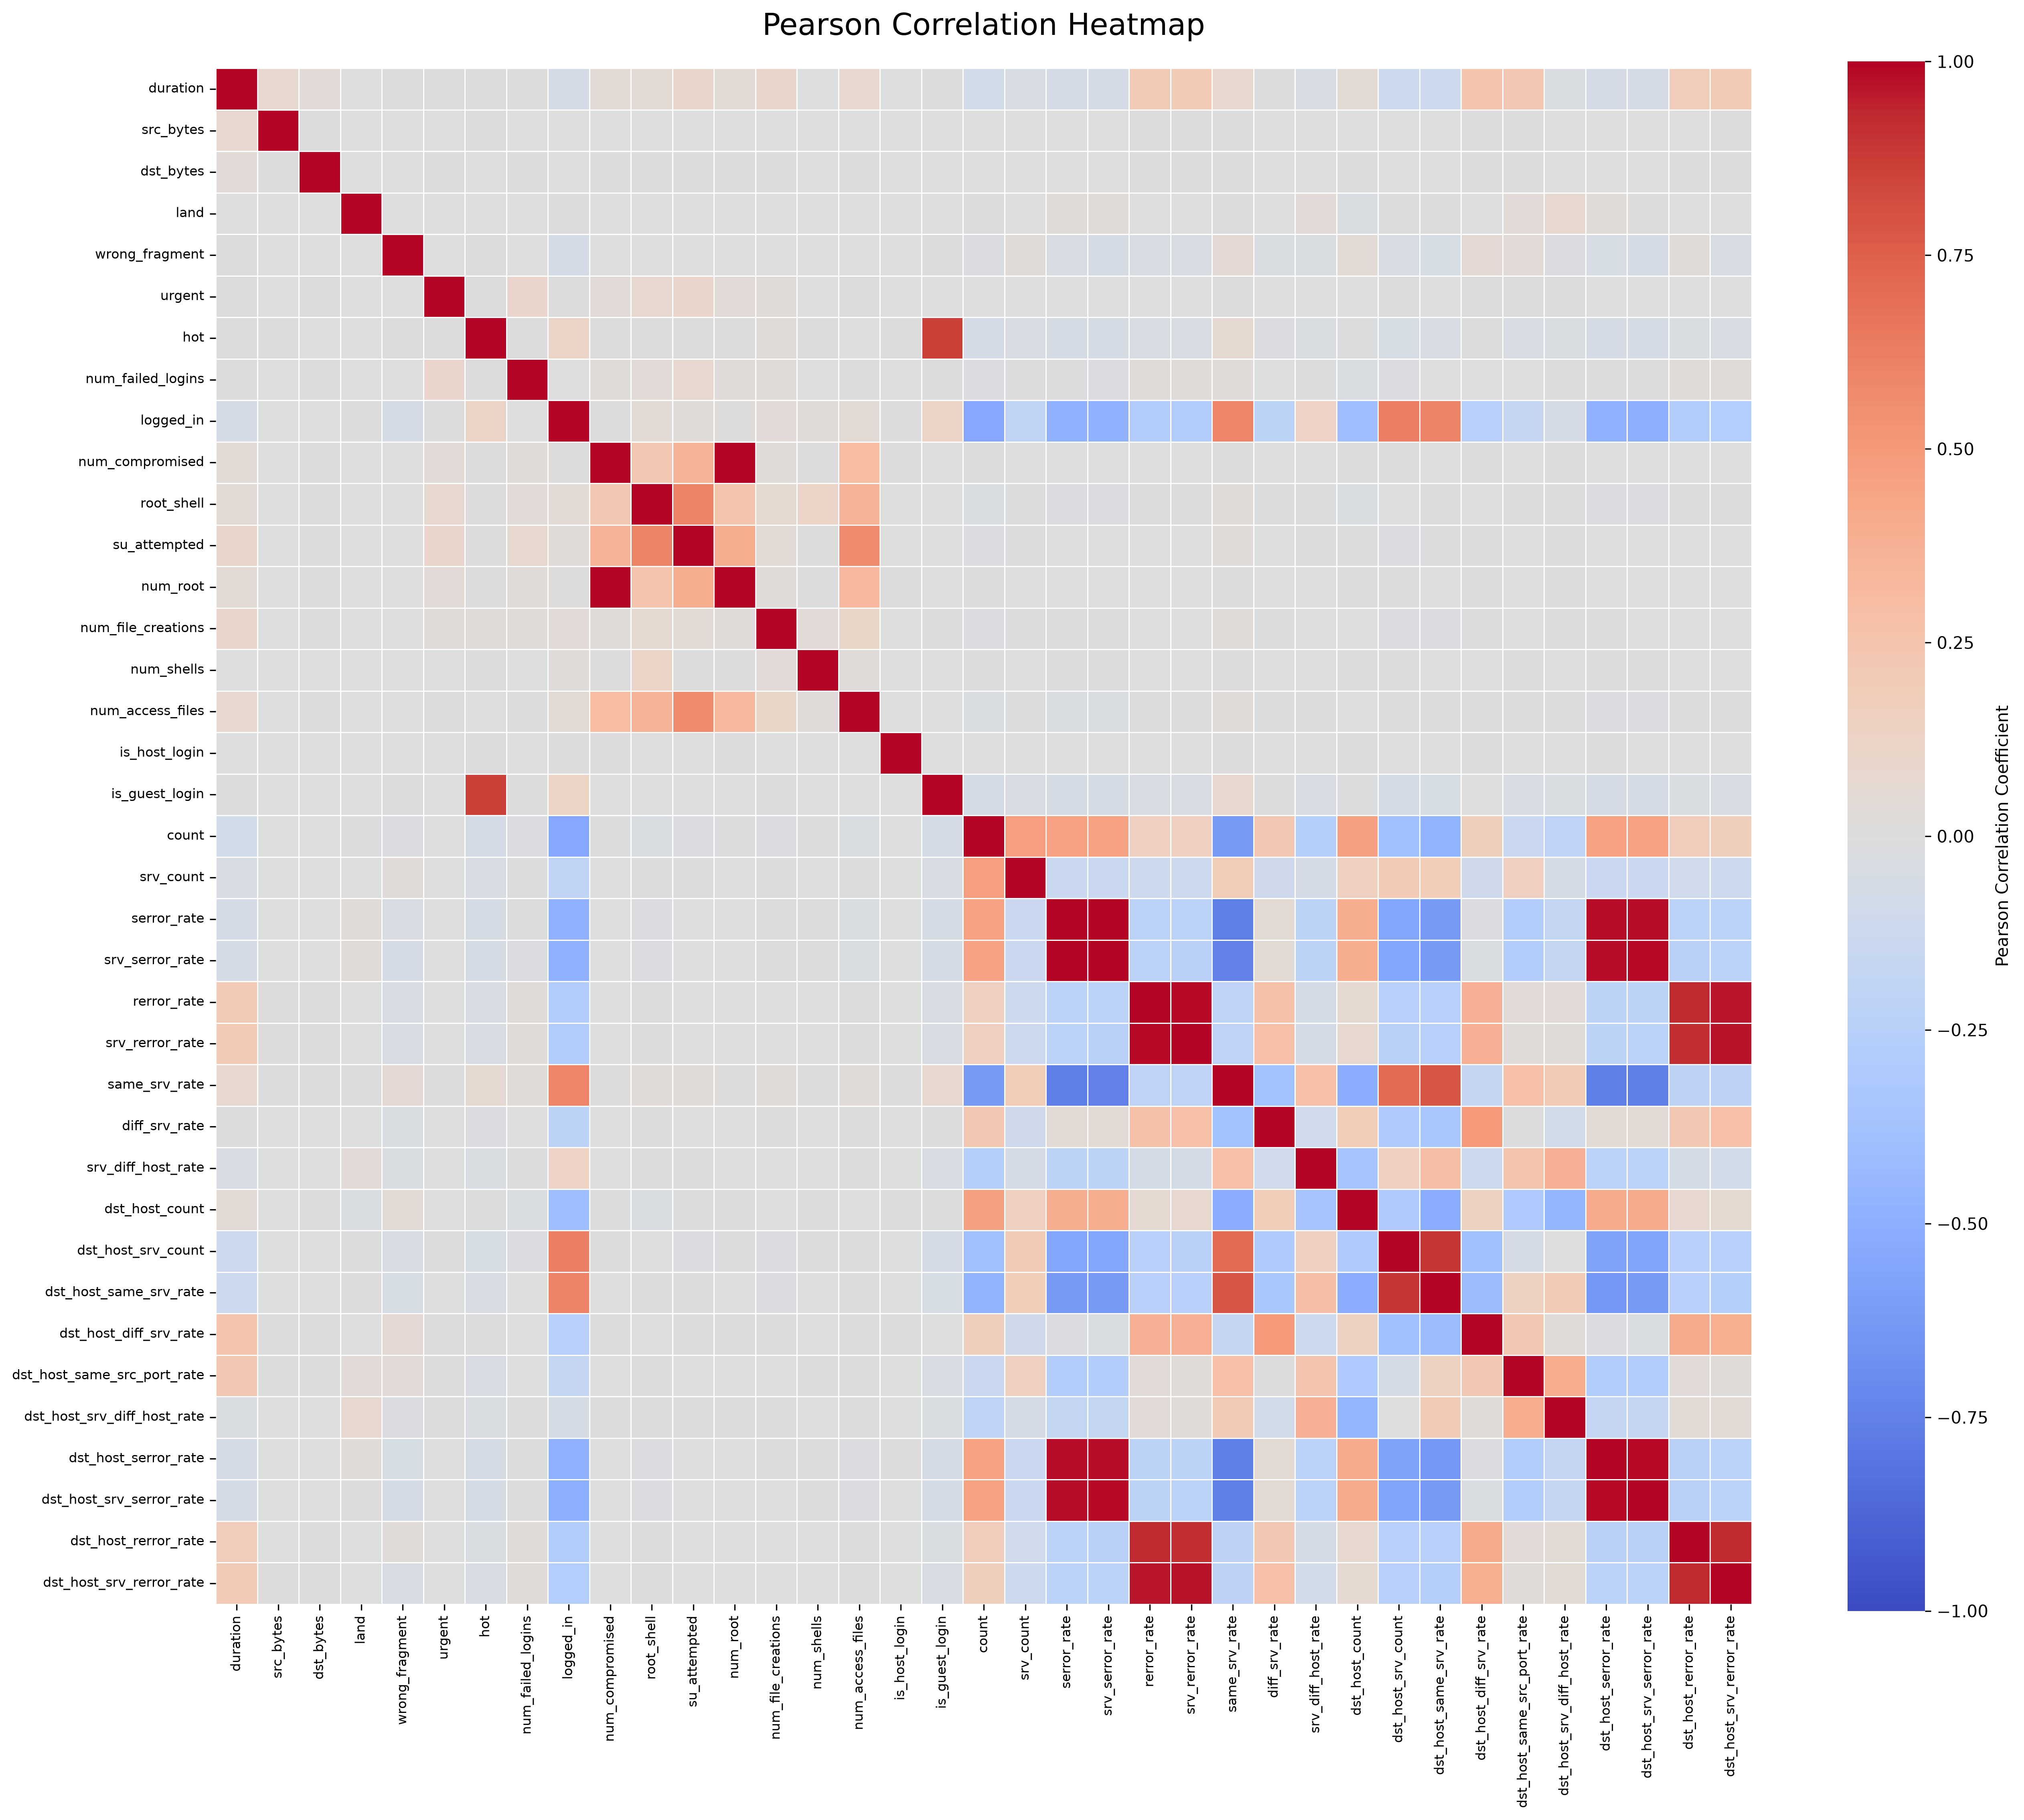
\includegraphics[width=0.78\linewidth]{outputs/pearson_heatmap.png}
\caption{Heatmap tương quan Pearson của 37 đặc trưng định lượng trong \url{train_clean.csv}.}
\label{fig:heatmap}
\end{figure}

Heatmap hỗ trợ nhận diện các cụm biến có quan hệ tuyến tính. Việc xác định cặp vượt ngưỡng được thực hiện bằng cách lọc hệ số trong ma trận, không chỉ dựa vào màu sắc của hình.

\section{Các cặp tương quan cao}
 
\hspace{0.4cm} Lọc tam giác trên của ma trận với điều kiện $|r|>0.95$ thu được 10 cặp. Tất cả đều tương quan thuận.

\begin{table}[htbp]
\centering
\caption{Các cặp đặc trưng có $|r|>0.95$}
\label{tab:highcorr}
\small
\begin{tabularx}{\linewidth}{
  >{\raggedright\arraybackslash}X
  >{\raggedright\arraybackslash}X
  r}
\toprule
Đặc trưng 1 & Đặc trưng 2 & $r$\\
\midrule
\url{num_compromised} & \url{num_root} & 0.998833\\
\url{serror_rate} & \url{srv_serror_rate} & 0.993289\\
\url{rerror_rate} & \url{srv_rerror_rate} & 0.989008\\
\url{srv_serror_rate} & \url{dst_host_srv_serror_rate} & 0.986252\\
\url{dst_host_serror_rate} & \url{dst_host_srv_serror_rate} & 0.985052\\
\url{serror_rate} & \url{dst_host_srv_serror_rate} & 0.981139\\
\url{serror_rate} & \url{dst_host_serror_rate} & 0.979373\\
\url{srv_serror_rate} & \url{dst_host_serror_rate} & 0.977596\\
\url{srv_rerror_rate} & \url{dst_host_srv_rerror_rate} & 0.970208\\
\url{rerror_rate} & \url{dst_host_srv_rerror_rate} & 0.964449\\
\bottomrule
\end{tabularx}
\end{table}

Trong 10 cặp, có 1 cặp liên quan đến biến đếm root, 6 cặp thuộc nhóm tỷ lệ lỗi SYN và 3 cặp thuộc nhóm tỷ lệ lỗi REJ. Kết quả chi tiết cũng được lưu tại \url{high_correlation_pairs.csv}.

\section{Phân tích khả năng dư thừa và kết luận}
 
\hspace{0.4cm} \textbf{Nhóm root:} \url{num_compromised} và \url{num_root} có $r=0.998833$. Theo từ điển dữ liệu, biến thứ nhất đếm các điều kiện compromised, còn biến thứ hai đếm số truy cập root. Tương quan gần hoàn hảo cho thấy liên hệ rất chặt, nhưng hai biến không đồng nghĩa về định nghĩa.

\textbf{Nhóm SYN:} \url{serror_rate}, \url{srv_serror_rate}, \url{dst_host_serror_rate} và \url{dst_host_srv_serror_rate} mô tả tỷ lệ lỗi SYN ở các phạm vi tổng hợp khác nhau. Sáu cặp có $r$ từ 0.977596 đến 0.993289, gợi ý khả năng trùng lặp một phần; khác biệt về phạm vi vẫn có thể mang thông tin riêng.

\textbf{Nhóm REJ:} \url{rerror_rate}, \url{srv_rerror_rate}, \url{dst_host_rerror_rate} và \url{dst_host_srv_rerror_rate} cùng phản ánh tỷ lệ lỗi REJ. Ba cặp có $r$ từ 0.964449 đến 0.989008. Tương tự nhóm SYN, tương quan cao là tín hiệu để xem xét chứ chưa đủ để kết luận biến có thể thay thế nhau.

Từ kết quả trên, đề xuất đưa 5 biến vào danh sách xem xét tiếp:
\begin{itemize}
  \item \url{num_root}
  \item \url{srv_serror_rate}
  \item \url{dst_host_srv_serror_rate}
  \item \url{srv_rerror_rate}
  \item \url{dst_host_srv_rerror_rate}
\end{itemize}
   
Đây không phải danh sách biến đã bị xóa. Pearson chỉ đo quan hệ tuyến tính; phân tích hiện tại chưa thử nghiệm mô hình trước/sau khi loại biến nên chưa thể kết luận ảnh hưởng đến hiệu suất dự đoán. Các tỷ lệ lỗi có miền $[0,1]$ và không phải phần trăm 0--100.

Tóm lại, phân tích trên 37 đặc trưng định lượng phát hiện 10 cặp có tương quan rất cao, tập trung ở ba nhóm root, SYN và REJ. Kết quả cung cấp bước sàng lọc ban đầu cho việc xem xét dư thừa thông tin; quyết định lựa chọn đặc trưng cần kết hợp định nghĩa biến, mục tiêu phân tích và đánh giá ở các bước tiếp theo.

\printbibliography[title={Tài liệu tham khảo}]
\end{document}
